%Since the NLO k-factors for $Z$ yields vary with $Z$ $p_T$, we estimated the impact on $\hat \mu$ of Higgs signal caused by imprecise modeling of $Z$ yield in different BDT regions. We perform a $Z$ injection test given the relative ratios $Z\rightarrow \mu \bar \mu$(Data) to \zmujets{}(MC). Asimov datasets were built with background function obtained from background only fit injecting $Z$ signal at strengths of these ratios multiplied by SM prediction while fixing the Higgs signal to be that of the SM. As discussed in~\ref{sec:fitbkgds}, the only \zjets{}nuisance parameter we adopt for the profile likelihood fit is a guassian constraint for the overall normalization. The bias of the $\mu_H$ is $\pm 10\%$ given the different ratios estimated with different MC \ref{tab:z_ratios}.% which is small enough and allow us to not include other nuisance parameters for $Z$ yield in different BDT regions. 

Both the ratio of data to MC for the \zmujets{} and the ratio of the \zmujets{} MC to \zjets{} MC have rather large deviations from 1 in some BDT regions.  Therefore we investigate the impact of changing the scaling the normalization of the $Z$ contribution in each BDT region from observed ratio of the number  data to MC for the \zmujets{} to the ratio of the number of events in \zmujets{} data to \zjets{} MC. While not a rigorous test of the scaling, it gives us a sense of the impact of the scaling on the sensitivity. These two sets of ratios are shown in Table~\ref{tab:z_ratios}. The overall normalization in both variations is fixed to be the data to MC from the \zmujets{}.  To compare these two sets of normalizations we do two injection tests.  Asimov datasets are built with the background function obtained from a background only fit while injecting the $Z$ signal  with the scalings shown in Table~\ref{tab:z_ratios}. Then, in the profile likelihood fit, the only \zjets{} nuisance parameter we adopt is a gaussian constraint for the overall normalization. The bias of the $\mu_H$ is $\pm 10\%$ given the different ratios estimated with different MC \ref{tab:z_ratios}.  This is quite small and gives us confidence that the fit results are not strongly influenced by the relative BDT region ratios.% which is small enough and allow us to not include other nuisance parameters for $Z$ yield in different BDT regions. 

The injection test using data to $Z\rightarrow b \bar b$ and $Z\rightarrow \mu \bar \mu$ MC ratios are shown in \ref{fig:Fit_combined_zbb} and \ref{fig:Fit_combined_zmm}.




\begin{table}[]
\centering
\caption{Relative Ratios of $Z\rightarrow \mu \bar \mu$(Data) to \zjets{}(MC) in each BDT region}
\label{tab:z_ratios}
\begin{tabular}{|l|r|r|}
\hline
Region       & $\frac{Z\rightarrow \mu \bar \mu(Data)}{Z\rightarrow b \bar b(MC)}$  &  $\frac{Z\rightarrow \mu \bar \mu(Data)}{Z\rightarrow \mu \bar \mu(MC)}$ \\ \hline
SRI (2cen)   & 1.89   & 0.80 \\ \hline
SRII (2cen)  & 1.20   & 1.90 \\ \hline
SRIII (2cen) & 0.67   & 0.57 \\ \hline
CR (2cen)    & 1.00   & 1.16 \\ \hline
SRI (4cen)   & 1.12   & 0.83 \\ \hline
SRII (4cen)  & 0.96   & 0.89 \\ \hline
CR (4cen)    & 1.03   & 1.17 \\ \hline

\end{tabular}
\end{table}

\begin{figure}[htbp]
  \centering
 \includegraphics[width=0.32\textwidth]{figures/FitCombined/zcheck_zdatazbb/zcheck_testVBF_ICHEP_2cen_SRI.pdf}
 \includegraphics[width=0.32\textwidth]{figures/FitCombined/zcheck_zdatazbb/zcheck_testVBF_ICHEP_2cen_SRII.pdf}
 \includegraphics[width=0.32\textwidth]{figures/FitCombined/zcheck_zdatazbb/zcheck_testVBF_ICHEP_2cen_SRIII.pdf}\\
 \includegraphics[width=0.32\textwidth]{figures/FitCombined/zcheck_zdatazbb/zcheck_testVBF_ICHEP_4cen_SRI.pdf}
 \includegraphics[width=0.32\textwidth]{figures/FitCombined/zcheck_zdatazbb/zcheck_testVBF_ICHEP_4cen_SRII.pdf}\\

\caption{$Z$ injection test with data to $Z\rightarrow b \bar b$ ratios. Fits from SR I to SR III (SR II) for 2 central (top) and 4 central (bottom) are shown.}
  \label{fig:Fit_combined_zbb}
\end{figure}


\begin{figure}[htbp]
  \centering
 \includegraphics[width=0.32\textwidth]{figures/FitCombined/zcheck_zdatazmm/zcheck_testVBF_ICHEP_2cen_SRI.pdf}
 \includegraphics[width=0.32\textwidth]{figures/FitCombined/zcheck_zdatazmm/zcheck_testVBF_ICHEP_2cen_SRII.pdf}
 \includegraphics[width=0.32\textwidth]{figures/FitCombined/zcheck_zdatazmm/zcheck_testVBF_ICHEP_2cen_SRIII.pdf}\\
 \includegraphics[width=0.32\textwidth]{figures/FitCombined/zcheck_zdatazmm/zcheck_testVBF_ICHEP_4cen_SRI.pdf}
 \includegraphics[width=0.32\textwidth]{figures/FitCombined/zcheck_zdatazmm/zcheck_testVBF_ICHEP_4cen_SRII.pdf}\\

\caption{$Z$ injection test with data to $Z\rightarrow \mu \bar \mu$ ratios. Fits from SR I to SR III (SR II) for 2 central (top) and 4 central (bottom) are shown.}
  \label{fig:Fit_combined_zmm}
\end{figure}
